%!TeX root=../../master.tex
\section{Gesture Recognition}\label{sec:gesturerecognition}
The system lets users control smart devices in their home by performing certain gestures.

Gesture recognition can generally be split into two categories: Camera-based and motion-based \cite{Kela2006}. Examples of camera-based gesture recognition systems are the ``Gesture Pendant'' \cite{starner2000gesture} and the Kinect \cite{kinect} and an example of a motion-based system is the Reemo \cite{Reemo}.

The camera-based solution require that the limbs used to perform gestures are visible to the camera and as such static cameras placed in a room may be rendered useless if the user turns his back against them. In addition, furniture and other people may stand in between them and obstruct the line of sight between the camera and the user.
This would likely not happen with the ``Gesture Pendant'', but the user would have to make sure that the pendant was always outside of any clothes worn as putting on a sweater or wrapping yourself in a blanket might block the view of the camera.

Motion-based solutions can employ various different sensors on the person, eg. accelerometers and gyroscopes and depending on the type of sensor different methods can be used to recognize gestures.
As mentioned in \Cref{sec:wearables} accelerometers are present in about half of the devices examined and therefore the motion-based solutions utilizing these will be the ones explored further.

\subsection{\$3 Gesture Recognizer}\label{sec:threedollar}
The \$3 Gesture Recognizer is a gesture recognition system created by Sven Kratz and Michael Rohs and is presented in the paper ``A \$3 Gesture Recognizer – Simple Gesture Recognition for Devices Equipped with 3D Acceleration Sensors'' \cite{threedollar}.

The system is based on the work of Wobrock et al. \cite{wobbrock2007gestures} and adds the ability to detect three dimensional gestures rather than being limited to two dimensional gestures.

Both of these systems are designed to be easy to use by anyone for fast prototyping of user interfaces which makes them appropriate for use in this project.
The \$3 Gesture Recognizer however would be better suited as it is capable of recognizing more gestures because it uses three-dimensional sensors.
This means that users have even more options for personalizing the gestures that they use to control their home with.

In addition, the \$3 Gesture Recognizer only requires the user to train a gesture about five times before it can deliver adequate recognition rates. This provides a better experience for the user as he does not need to spend much time training the system before he is able to use it.

The way the \$3 Gesture Recognizer works is by collecting data from a three-axis accelerometer and from this it creates a gesture trace $T$ which consists of a set of candidate points, this is illustrated in \Cref{fig:onedollar-gesturetrace}.
Also shown in this figure is that the gesture traces can contain a different number of points when performing the same gesture at different speeds.
Because of this, the \$3 Gesture Recognizer resamples $T$ so that it contains a fixed number of points, in \cite{threedollar} it's $N = 150$, with equal distance between the points.
If $N$ is set to a lower value, then precision is lost, but if $N$ is set to a higher value, then computational cost increases.
After resampling the points, $T$ is rotated in an attempt to correct for any rotational error and finally it is scaled to fit inside of a cube of $100^3$ units to compensate for the fact that may perform inconsistently sized gestures.

Once all of these modifications have been performed, the gesture trace is matched against all the training gestures\footnote{Whenever a user trains a gesture, a new gesture trace is stored and associated with a gesture class. A gesture class that has been trained five times hence has five gesture traces stored.}.
From these comparisons a scoring table is created where each training gesture is scored based on the distance between it and the input gesture trace. To reduce the amount of false positives a scoring heuristic is used, which simply determines whether a score is above a threshold $\epsilon$.

\begin{figure}[!htb]
  \centering
  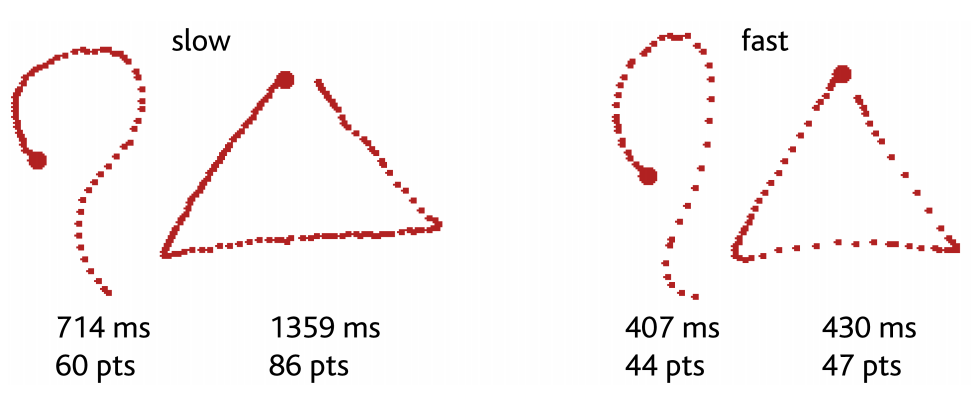
\includegraphics[width=0.8\textwidth]{images/1-dollar-gesturetrace.png}
  \caption[Some Caption]{``A slow and fast question mark and triangle made by
subjects using a stylus on a Pocket PC. Note the considerable time
differences and resulting numbers of points''\footnotemark}
\label{fig:onedollar-gesturetrace}
\end{figure}
\footnotetext{Image and text is from Figure 3 in \cite{wobbrock2007gestures}}

\subsection{Detecting Points Before and After Gestures}

Before a user performs a gesture in order to control an actuator, he must point at the actuator he desires to control. A point is defined as the user holding his phone still for a period of time. An accelerometer can be used to detect if the user holds the device still. If there is a low amount of activity on all three axis, it is assumed that the user is holding the device in his hand without moving it.

Figure \ref{fig:gesture-recognition:point-to-gesture-state-diagram} shows the relationship of a point and a gesture in a state diagram. All gestures begin and end with a point. When the first point is detected, a very short delay is introduced in order for the user to prepare to do the gesture, e.g. move the position of his hand. When the delay has passed, the gesture recognition begins. Gestures are recognized using the previously described \$3 Gesture Recognizer. After the gesture has been performed, the device must be held still again and the second point is detected. The collected gesture data is then analyzed by \$3 Gesture Recognizier in order to determine which known gesture was performed, if any at all. Lastly, the system returns to the initial state and another gesture can be performed.

While performing the gesture, the recognition may timeout. The \$3 Gesture Recognizer has can recognize gestures for a maximum of four seconds before the recognition is cancelled. In such case, the system returns to the initial state.

\begin{figure}[h]
\centering
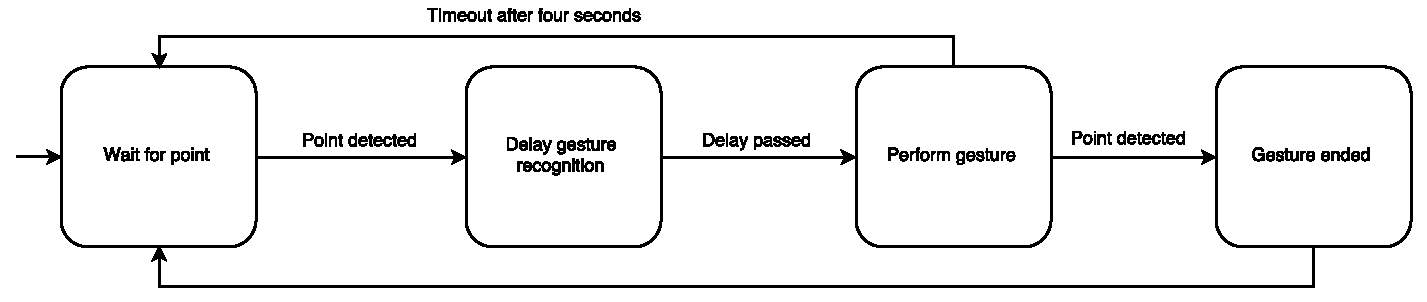
\includegraphics[width=\textwidth]{images/point-to-gesture-state-diagram}
\label{fig:gesture-recognition:point-to-gesture-state-diagram}
\caption{State diagram showing the relationship between a point and a gesture. A gesture always starts and ends with a point.}
\end{figure}

\subsubsection{Using Accelerometer Data to Detect a Point}

Figure \ref{fig:gesture-recognition:pointer} shows screenshots of an application created to experiment with data from the accelerometer. The figure shows graphs of measurements made while the device was lying on a table, the user was pointing with the device in his hand and while the user was walking with the device in his hand. $x$-, $y$- and $z$-values are measued in radians per second. The $y$-axis of the graph spans from -5 to 5. The graphs shows that there are small but measureable differences between the measurements made while a device is lying on the table and the user is pointing with the device. This allows us to distinct between the two scenarios and disregard measurements made while the device is lying on the table.

Furthermore the graphs clearly shows that there is a measurable difference between the values read when a user is pointing with a device and walking with the device in his hand. Based on the small experiment we can conclude that the accelerometer data can be used to determine if a user is pointing with a device.

\begin{figure}[!htb]%
    \centering
    \subfloat{
        \frame{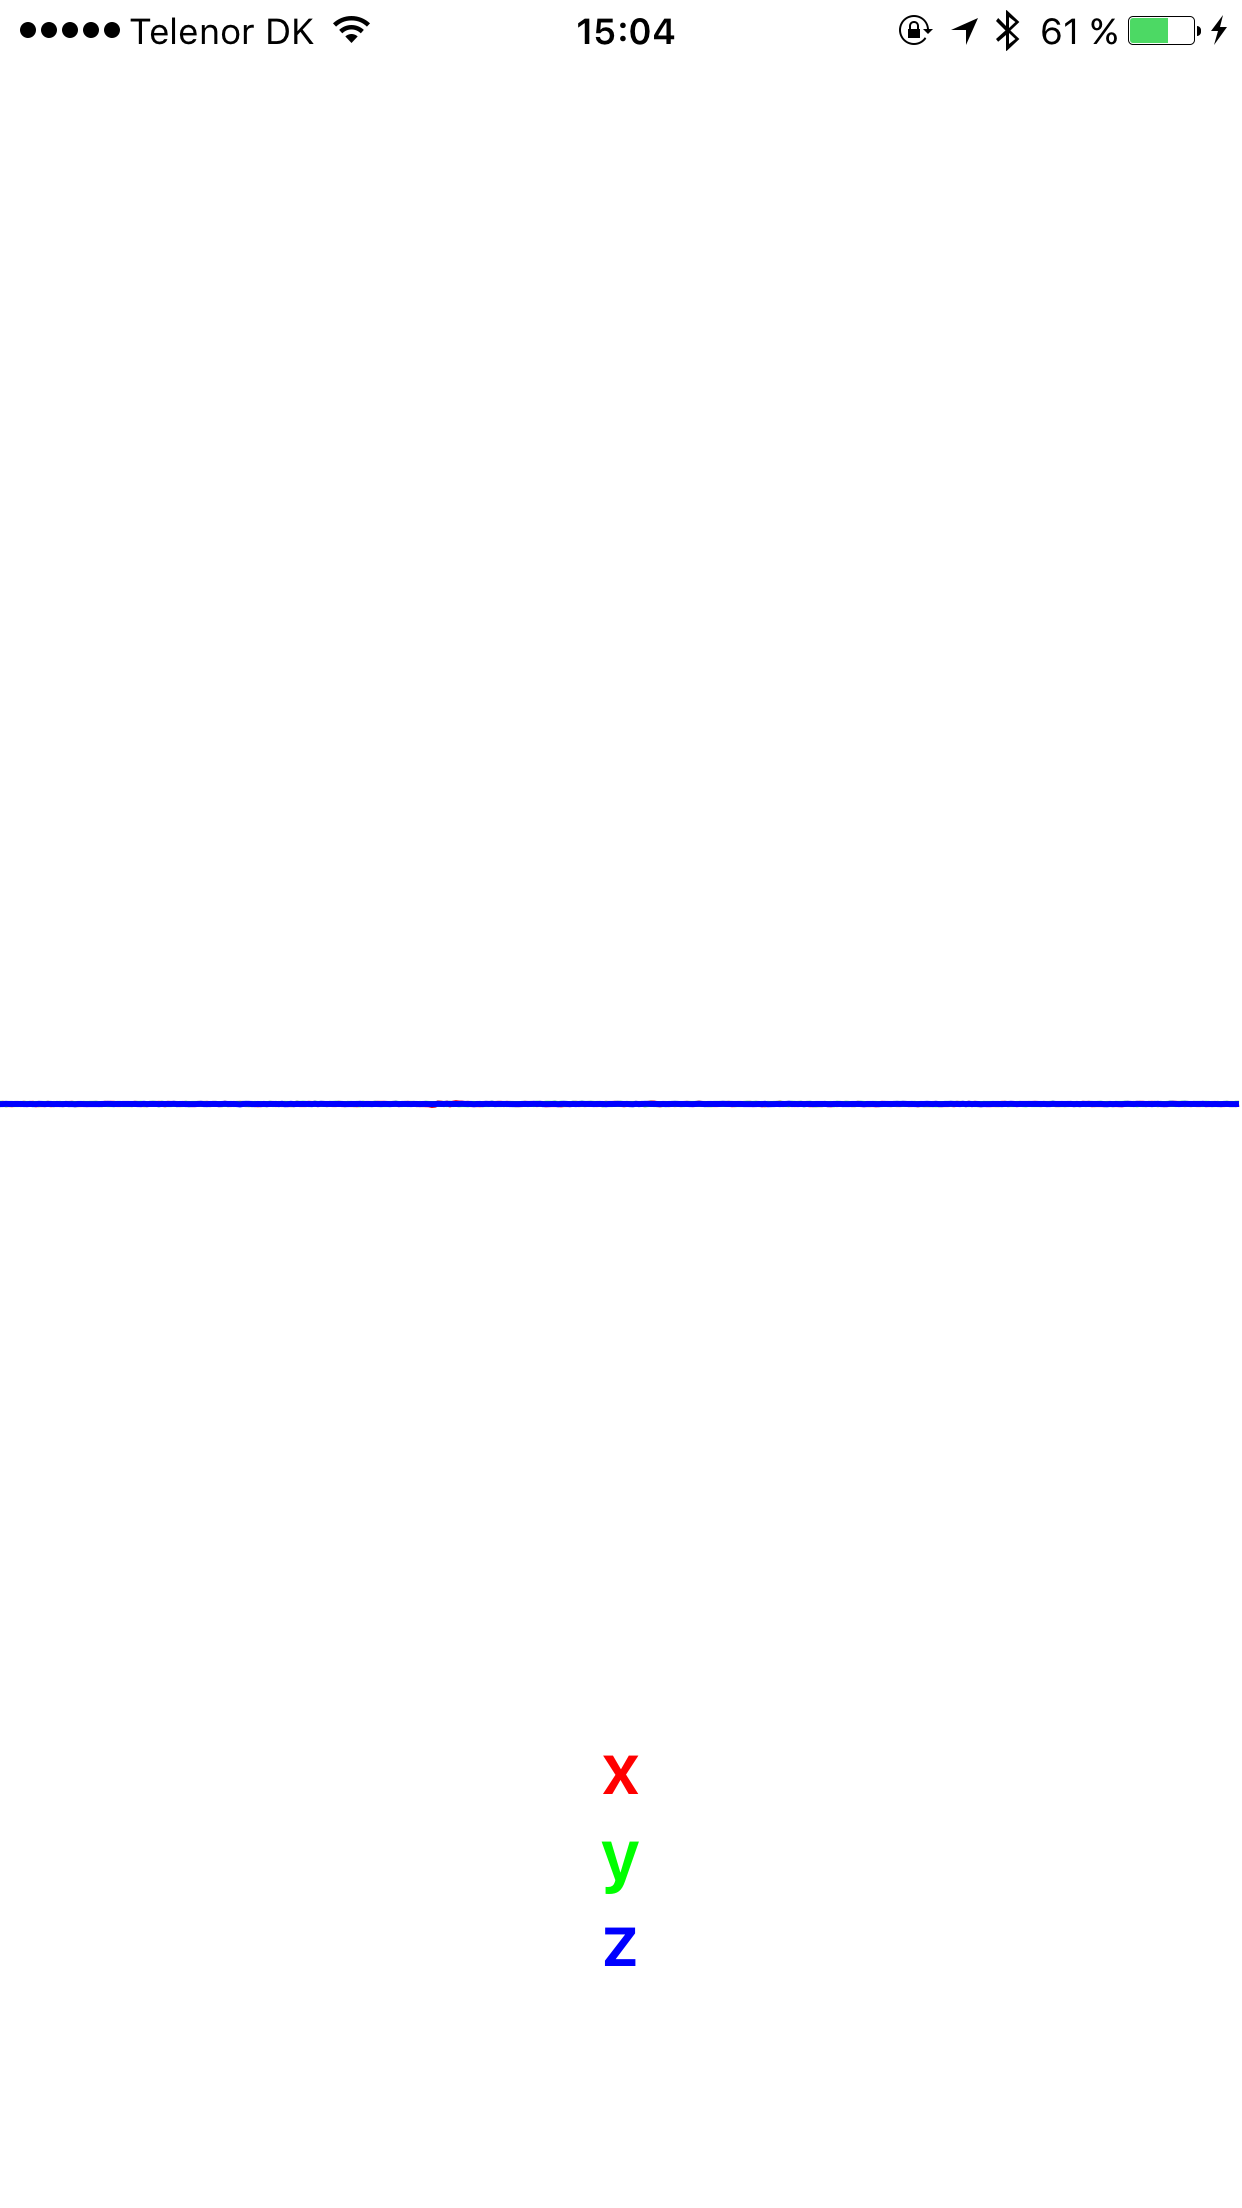
\includegraphics[width=0.3\textwidth]{images/pointer-table}}
    }
    \subfloat{
        \frame{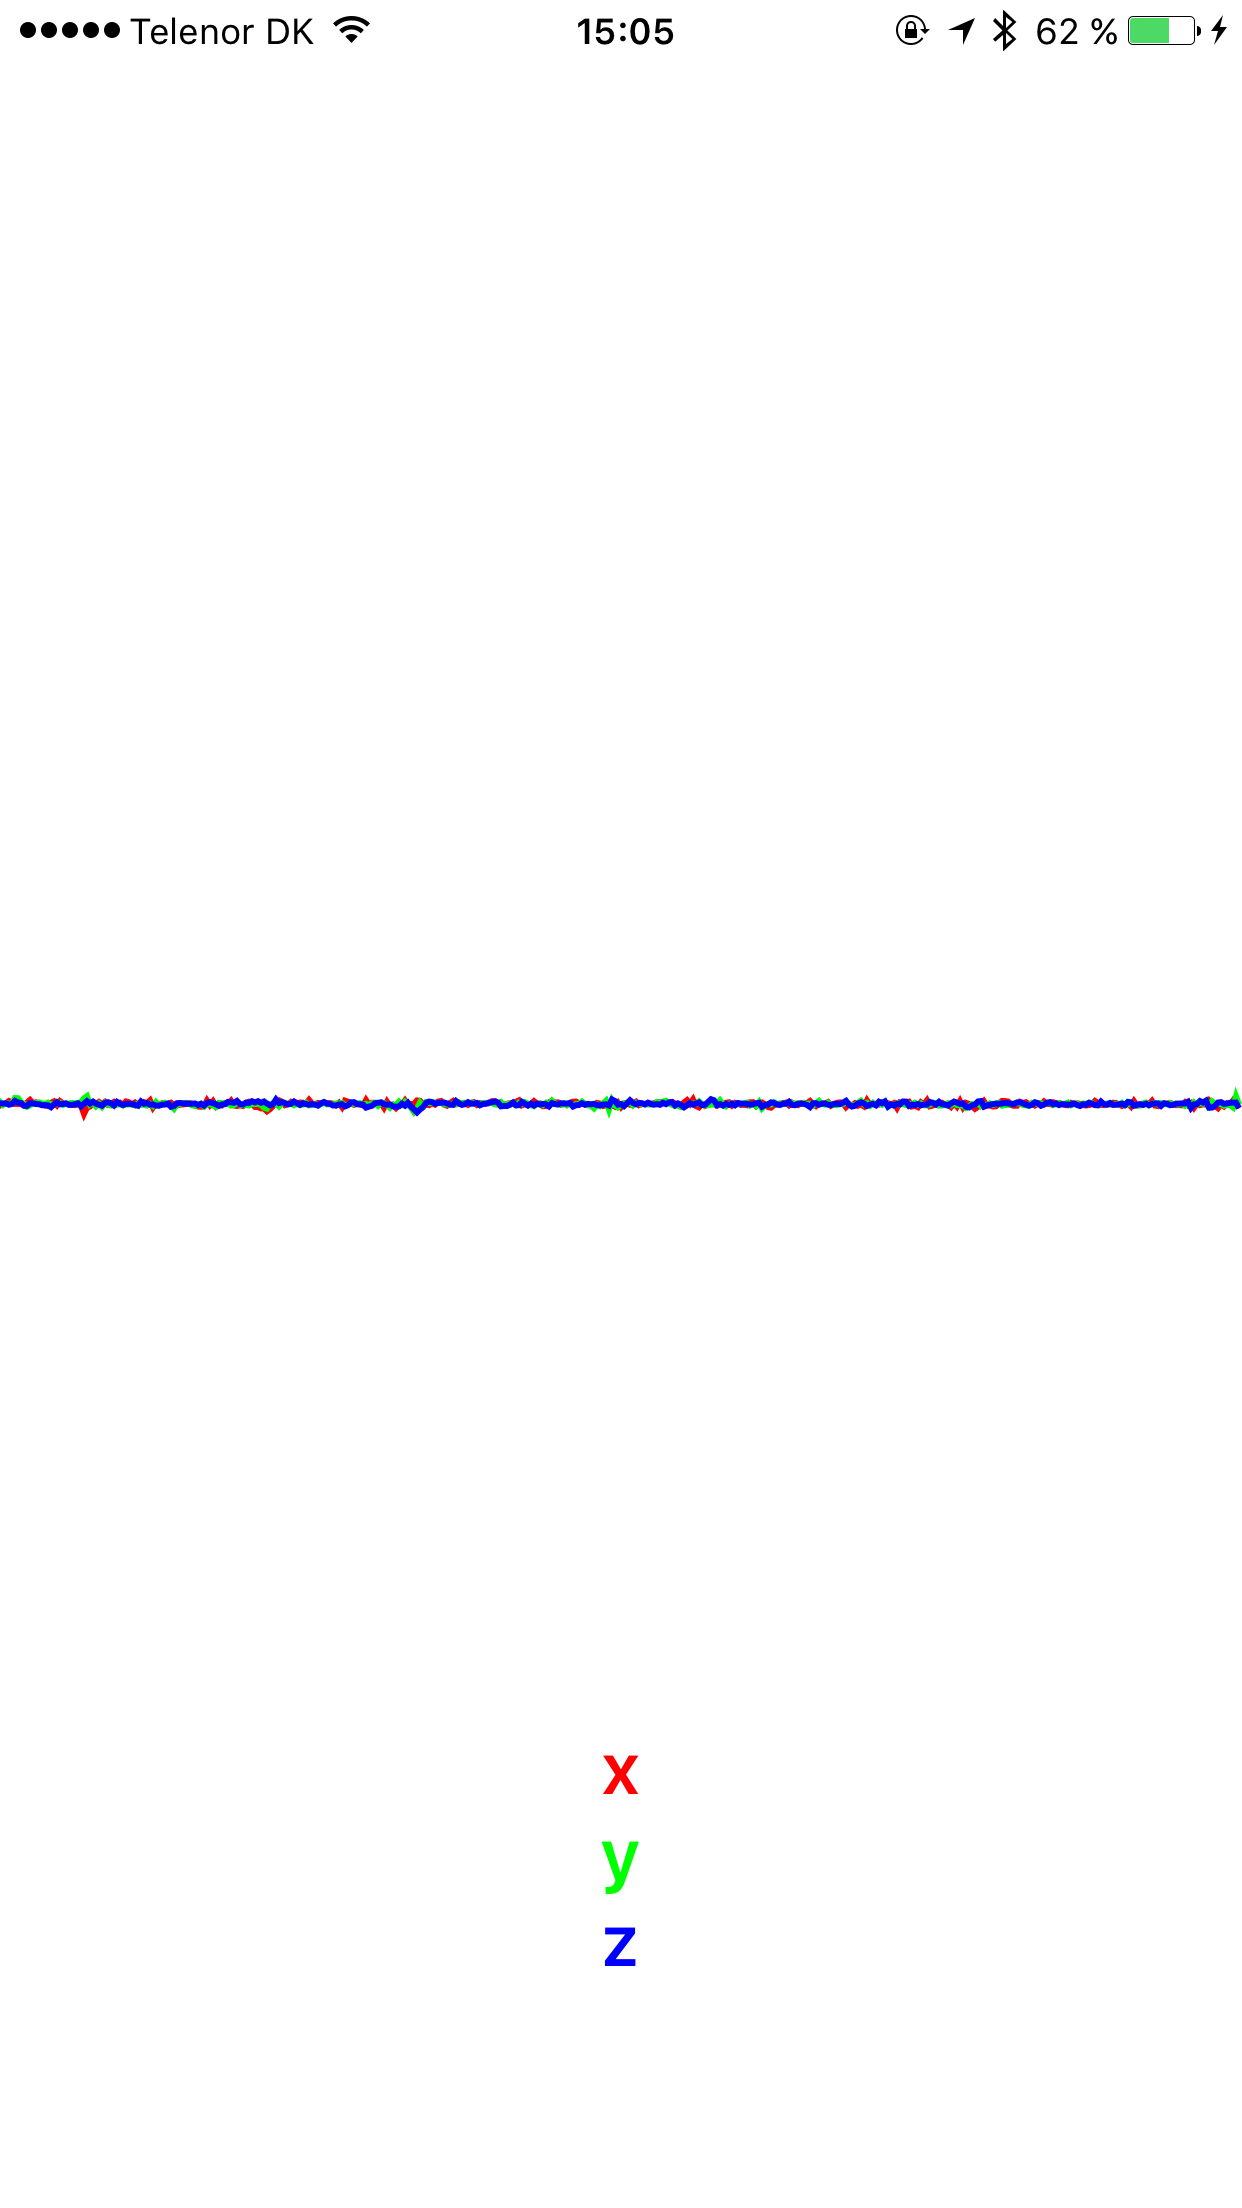
\includegraphics[width=0.3\textwidth]{images/pointer-hand}}
    }
    \subfloat{
        \frame{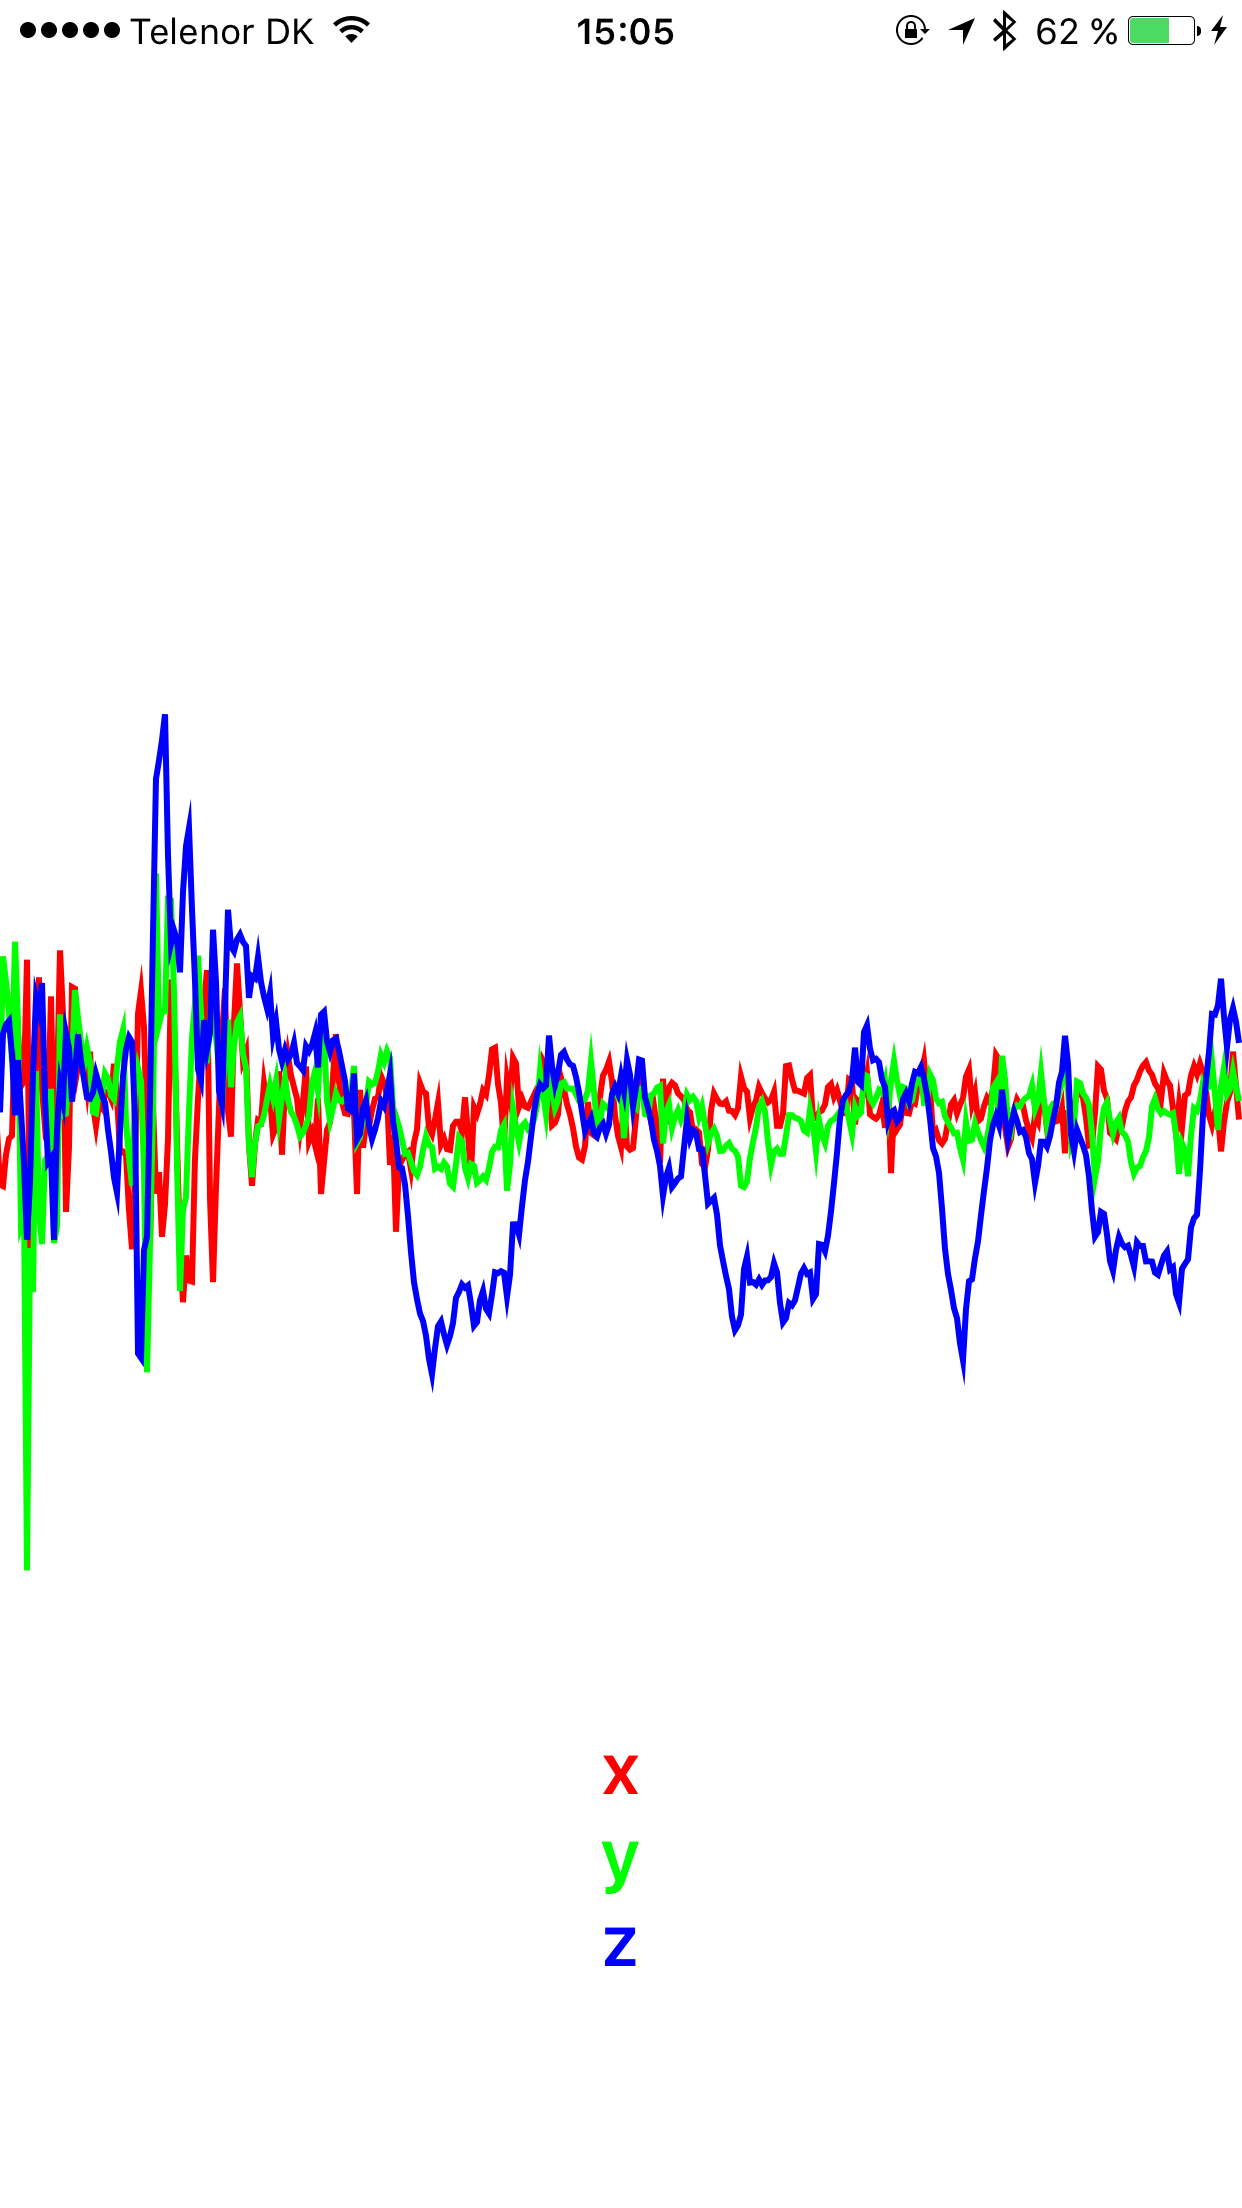
\includegraphics[width=0.3\textwidth]{images/pointer-walk}}
    }
    \caption{Screenshots of application created to experiment with data from the accelerometer. Leftmost screenshot shows graph of measurements made when the device lies on a table. The middle image shows graph of measurements made while pointing with the device. Rightmost screenshot shows graph of measurements made while the user was walking with the device in his hand.}
    \label{fig:gesture-recognition:pointer}
\end{figure}

\subsubsection{Detecting Points using PointDetector}

\begin{figure}
\centering
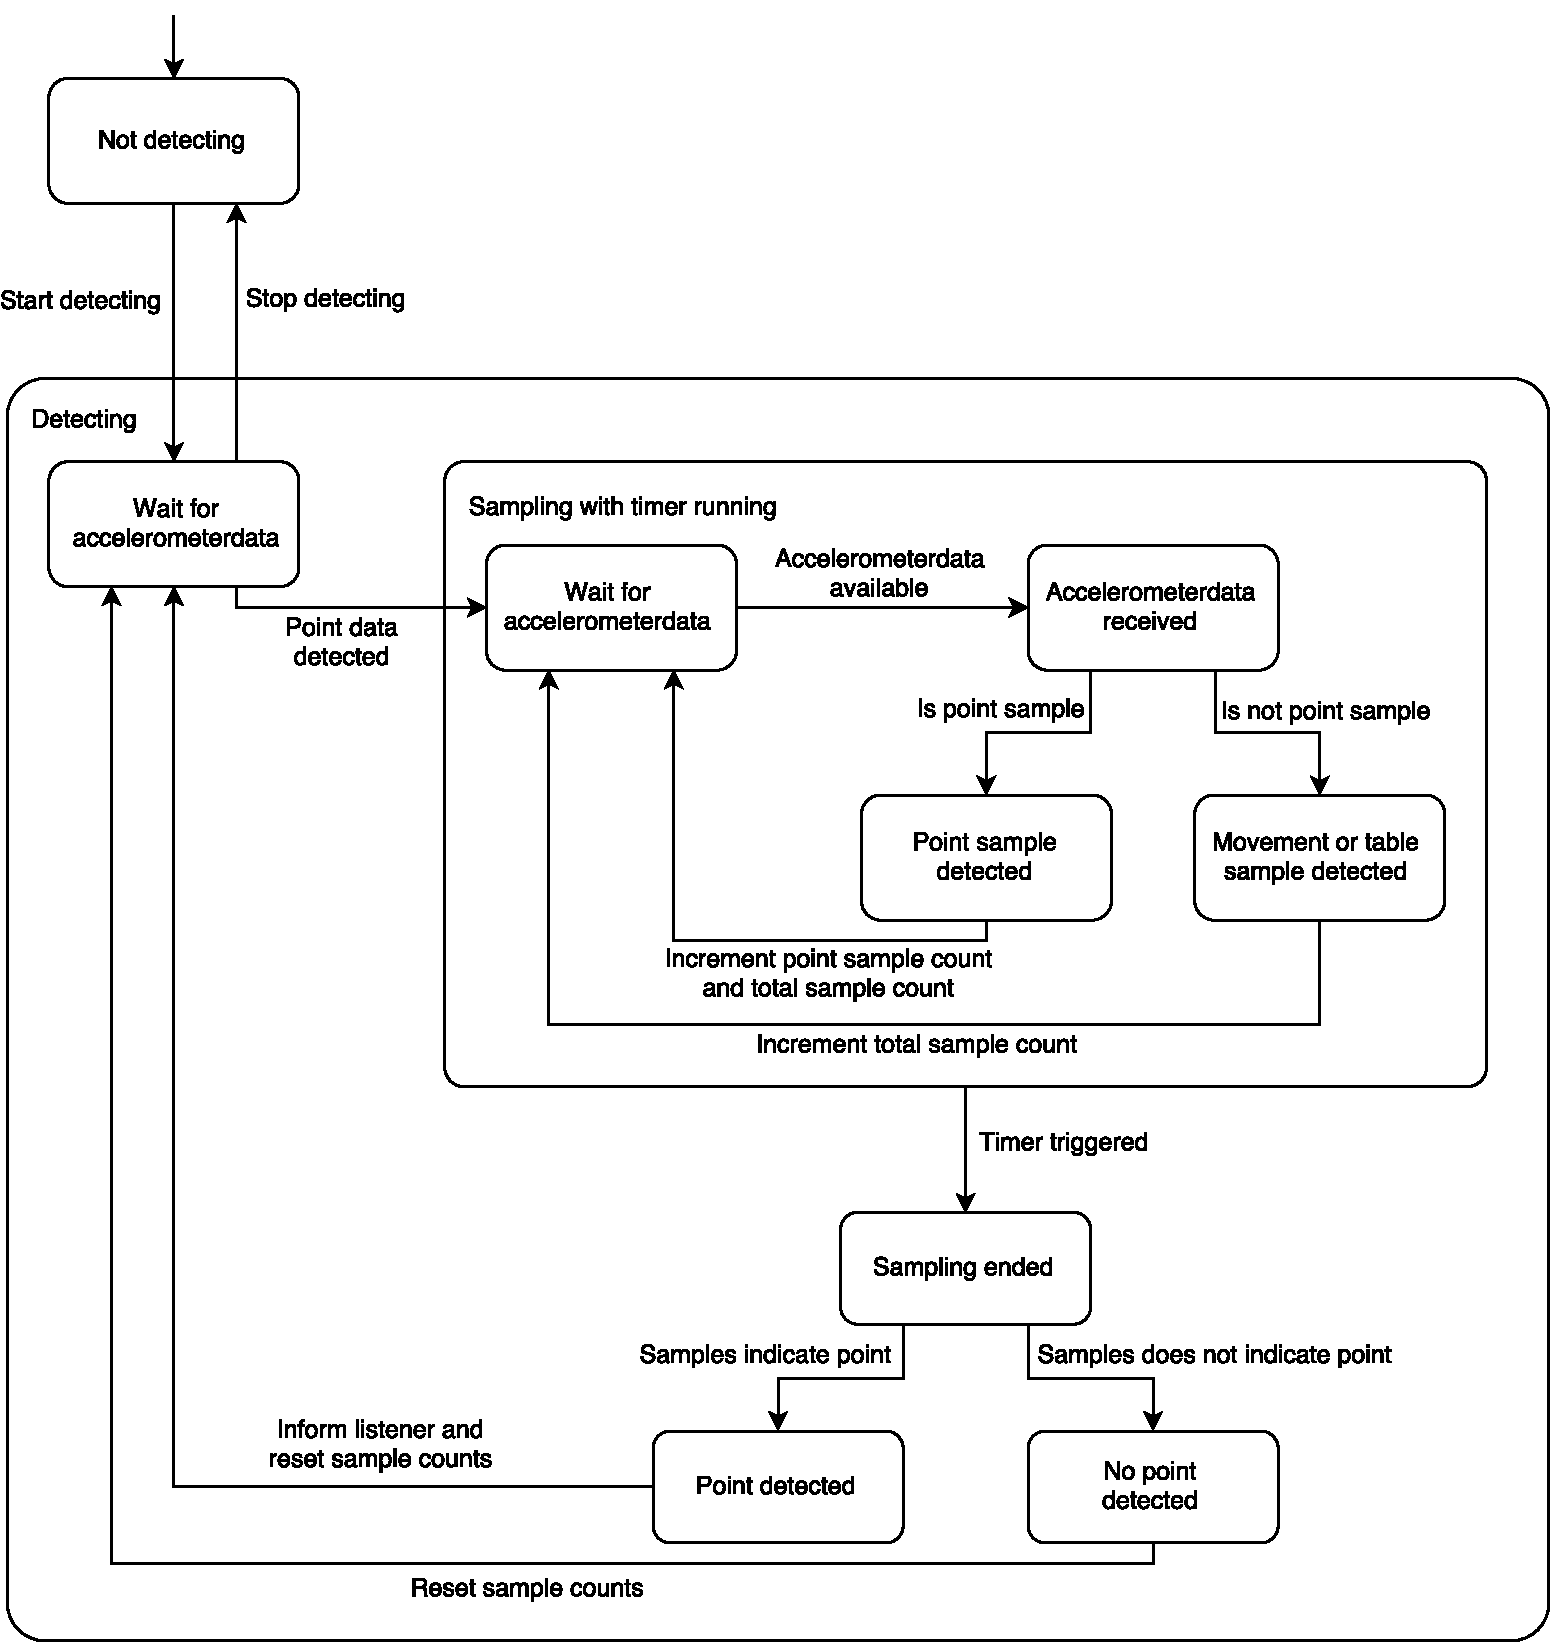
\includegraphics[width=\textwidth]{images/point-detector-state-diagram}
\label{fig:gesture-recognition:pointdetector-state-diagram}
\caption{State diagram showing the states the \texttt{PointDetector} class can be in.}
\end{figure}

\begin{figure}
\centering
\begin{tikzpicture} 
\umlclass[x=0,y=0]{PointDetector}{
+/- isDetecting: Bool\\
- isSampling: Bool\\
- pointingDuration: Float\\
- pointingSampleFrequency: Float\\
- pointingThreshold: Float\\
- tableThreshold: Float\\
- samplingTimer: Timer\\
- pointingSampleCount: Int\\
- totalSampleCount: Int\\
- pointDetectedCallback: Closure?
}{
+ beginDetecting()\\
+ endDetecting()\\
- didUpdateMotionData(data: AccelerometerData)\\
- isMotionDataAPointingGesture(data: AccelerometerData): Bool\\
- dataFitsWithinThreshold(data: AccelerometerData, threshold: Double): Bool\\
- samplingTimerTriggered()
} 
\end{tikzpicture}
\label{fig:gesture-recognition:pointdetector-uml}
\caption{Class diagram of the \texttt{PointDetector} class.}
\end{figure}

%%% Local Variables:
%%% mode: latex
%%% TeX-master: "../../master"
%%% TeX-command-extra-options: "-shell-escape"
%%% End:
